\subsection{Nascent IFIT1, IFIT3, and IFIT5 Localisation in a Simplified System of pseudo-IBs} \label{subsec:Nascent IFIT1, IFIT3, and IFIT5 Localisation in a Simplified System of pseudo-IBs}
\subsubsection{pIB IFIT1}

\begin{figure}
    \begin{subfigure}{0.495\textwidth}
        \caption{}
        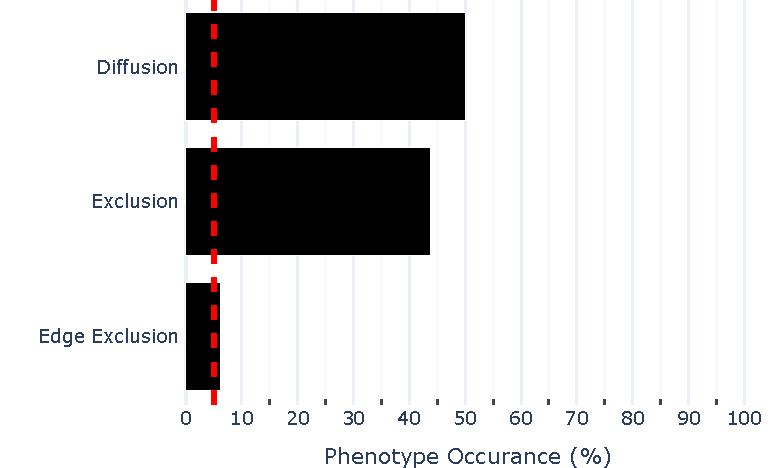
\includegraphics[width=1\linewidth]{09. Chapter 4/Figs/03. pIB/01. IFIT1/01. bar_i1_293t.pdf} 
    \end{subfigure}
    \begin{subfigure}{0.495\textwidth}
        \caption{}
        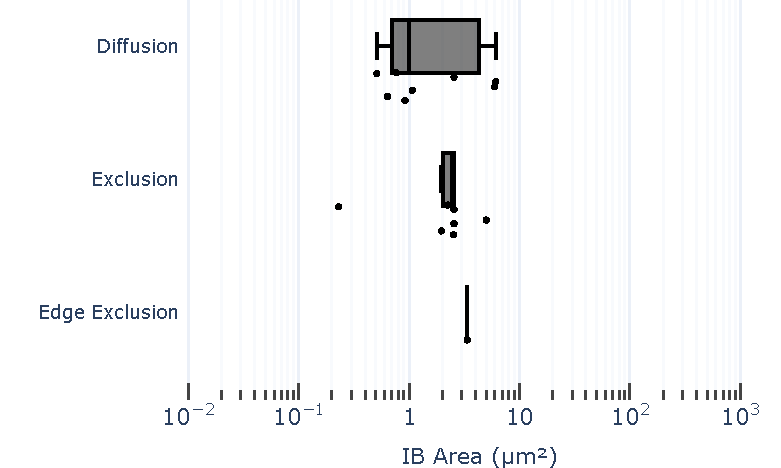
\includegraphics[width=1\linewidth]{09. Chapter 4/Figs/03. pIB/01. IFIT1/02. box_i1_293t.pdf}
    \end{subfigure}
    \begin{subfigure}{1\textwidth}
        \centering
        \caption{}
        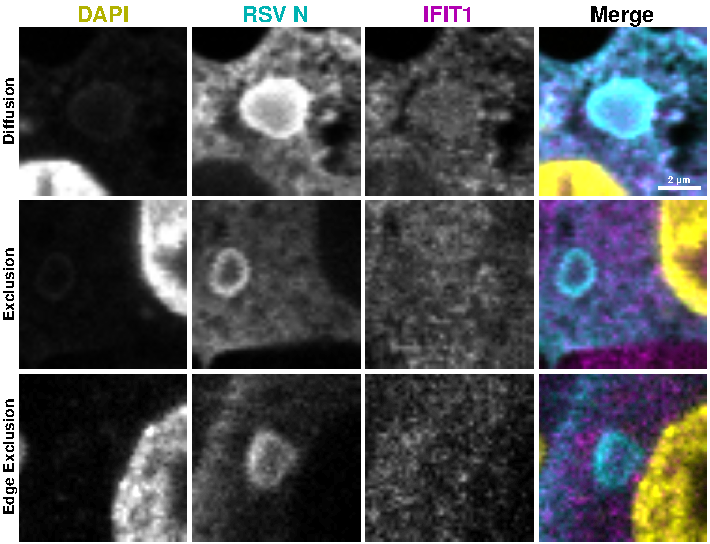
\includegraphics[width=1\linewidth]{09. Chapter 4/Figs/03. pIB/01. IFIT1/03. i1-293t-hnhp.pdf}
    \end{subfigure}
    \caption[i1 293t hnhp]{\textbf{i1 293t hnhp.} 16}
    \label{fig:i1 293t hnhp}
\end{figure}

Nascent human IFIT1 seems to be diffused through the pIB structure i.e., the signal intensity and distribution between cytoplasmic and pIB staining is identical.  

Endogenous monkey IFIT1 displays colocalization with human pIB structures (top panel), or inclusion within the structures (bottom panel). Monkey IFIT1 signal is also excluded from the pIB filamentous network (top panel; shown by arrows). This suggests that the colocalization is not caused by mere interaction with N or P but its dependant on the integrity of pIBs. These data are supported by z stack measurements.  

\begin{figure}
    \begin{subfigure}{0.495\textwidth}
        \caption{}
        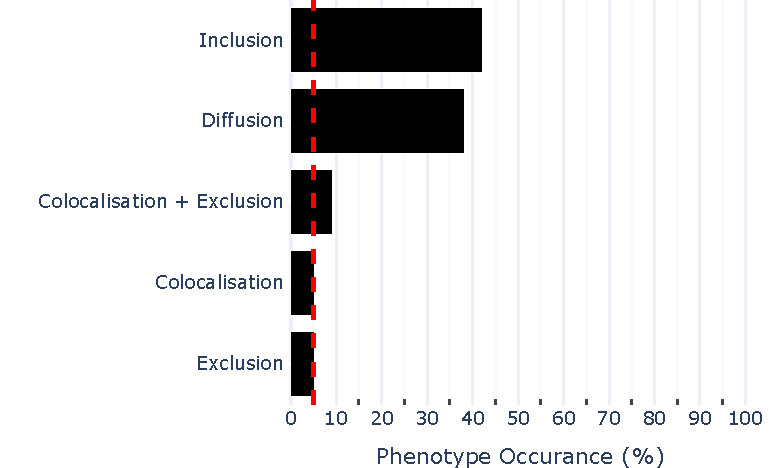
\includegraphics[width=1\linewidth]{09. Chapter 4/Figs/03. pIB/01. IFIT1/04. bar_i1_vero_hnhp.pdf} 
    \end{subfigure}
    \begin{subfigure}{0.495\textwidth}
        \caption{}
        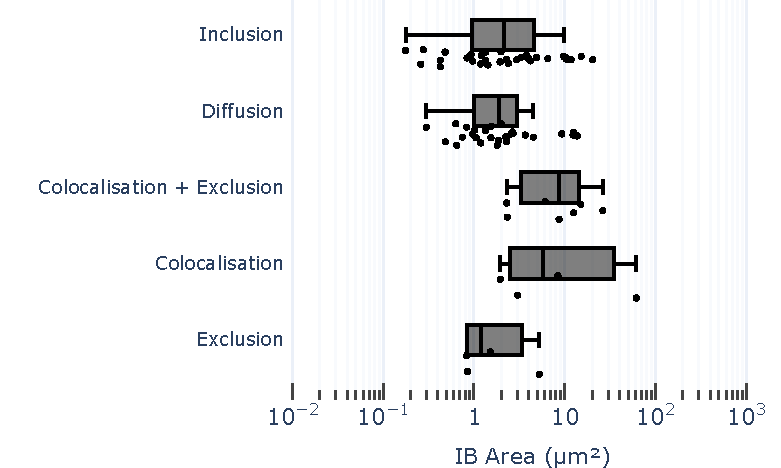
\includegraphics[width=1\linewidth]{09. Chapter 4/Figs/03. pIB/01. IFIT1/05. box_i1_vero_hnhp.pdf}
    \end{subfigure}
    \caption[i1 vero hnhp plots]{\textbf{i1 vero hnhp plots.} 76}
    \label{fig:i1 vero hnhp plots}
\end{figure}

\begin{figure}
    \centering
    \includegraphics[width=1\linewidth]{09. Chapter 4/Figs/03. pIB/01. IFIT1/06. i1-vero-hnhp.pdf}
    \caption[i1 vero hnhp]{\textbf{i1 vero hnhp.} Nascent bovine IFIT1 in the context of bRSV infection has been observed to localise with the respect of IB in three distinct spaces. We observed it either concentrated inside the central point of the IB structure, while having reduced signal on the inner IB edge, compared to the cytoplasm (top and bottom panels), being excluded from the IB structure (3rd panel), or colocalising on the inner edge of the IB structure while having reduced signal in the middle of the structure compared to cytoplasm, or the edge staining (2nd panel).}
    \label{fig:i1 vero hnhp}
\end{figure}

In the context of bovine pIB structures, nascent monkey IFIT1 seems to colocalise with the edges of the structures (highlighted by the arrows). Consistent to human pIB data, nascent monkey IFIT1 is excluded from filamentous pIB network.

\begin{figure}
    \begin{subfigure}{0.495\textwidth}
        \caption{}
        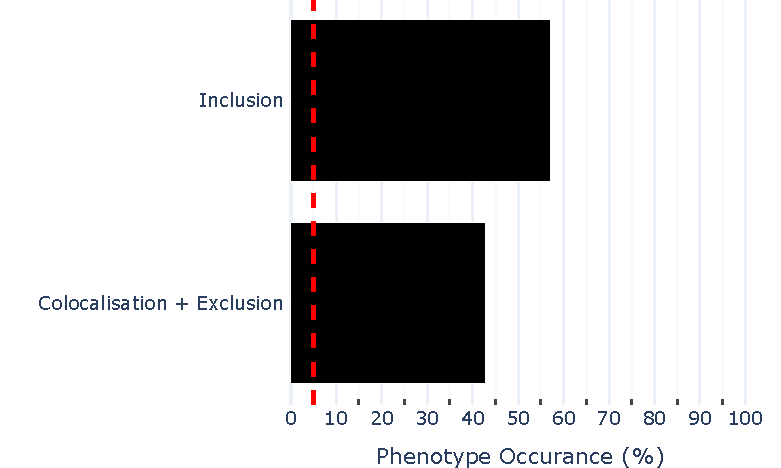
\includegraphics[width=1\linewidth]{09. Chapter 4/Figs/03. pIB/01. IFIT1/07. bar_i1_vero_bnbp.pdf} 
    \end{subfigure}
    \begin{subfigure}{0.495\textwidth}
        \caption{}
        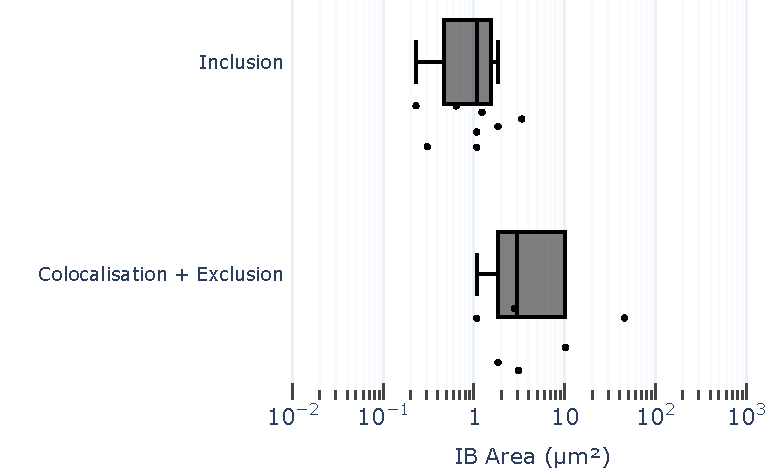
\includegraphics[width=1\linewidth]{09. Chapter 4/Figs/03. pIB/01. IFIT1/08. box_i1_vero_bnbp.pdf}
    \end{subfigure}
    \begin{subfigure}{1\textwidth}
        \centering
        \caption{}
        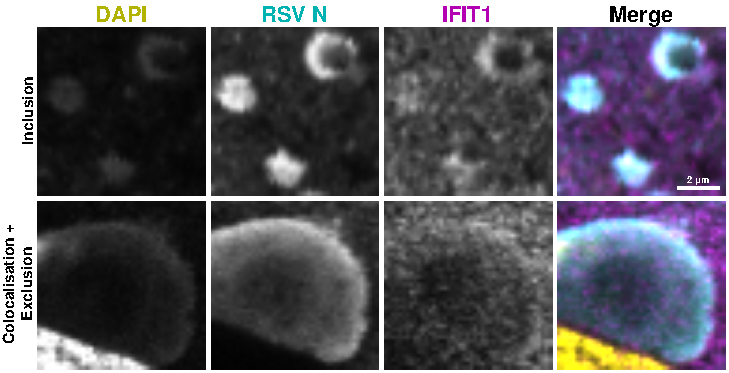
\includegraphics[width=1\linewidth]{09. Chapter 4/Figs/03. pIB/01. IFIT1/09. i1-vero-bnbp.pdf}
    \end{subfigure}
    \caption[i1 vero bnbp]{\textbf{i1 vero bnbp.} 14}
    \label{fig:i1 vero bnbp}
\end{figure}

\subsubsection{pIB IFIT3}
Nascent monkey IFIT3 seems to behave a if he pIB was not here. This means I has diffused phenotype. One exception is the top panel (shown with the arrow) which hints at concentrated IFIT3 at the edge of the pIBs. We do not know the localisation with respect to the pIB filaments as none were found in the slides. This data is as well supported by z stack measurements.

\begin{figure}
    \begin{subfigure}{0.495\textwidth}
        \caption{}
        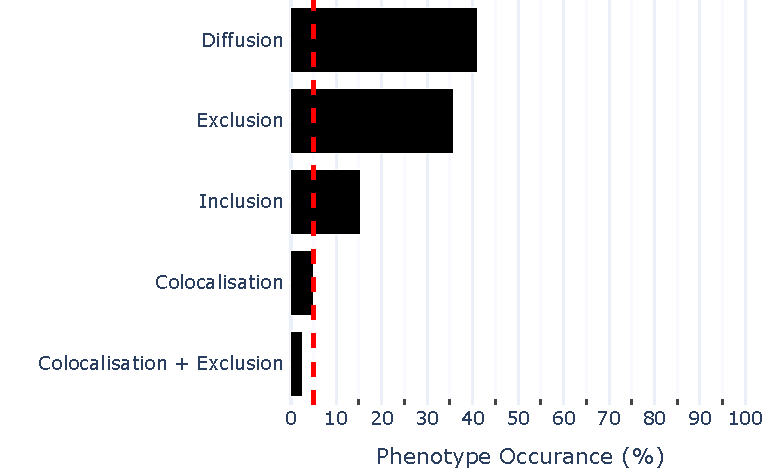
\includegraphics[width=1\linewidth]{09. Chapter 4/Figs/03. pIB/02. IFIT3/01. bar_i3_vero.pdf} 
    \end{subfigure}
    \begin{subfigure}{0.495\textwidth}
        \caption{}
        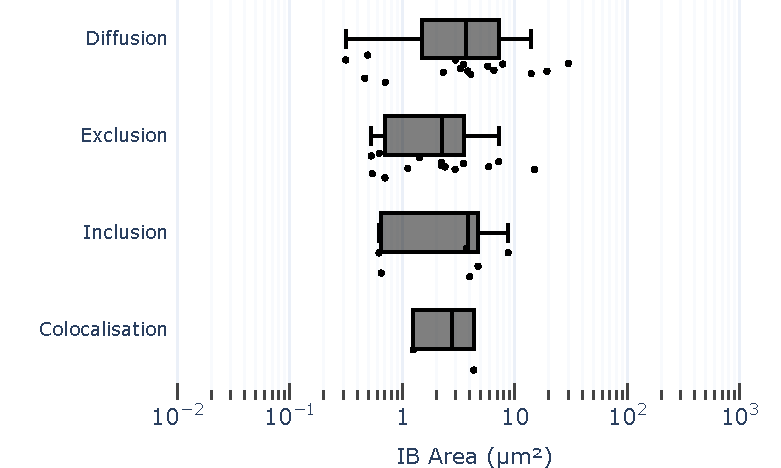
\includegraphics[width=1\linewidth]{09. Chapter 4/Figs/03. pIB/02. IFIT3/02. box_i3_vero.pdf}
    \end{subfigure}
    \caption[i3 vero hnhp plots]{\textbf{i3 vero hnhp plots.} 39}
    \label{fig:i3 vero hnhp plots}
\end{figure}

\begin{figure}
    \centering
    \includegraphics[width=1\linewidth]{09. Chapter 4/Figs/03. pIB/02. IFIT3/03. i3-vero-hnhp.pdf}
    \caption[i3 vero hnhp]{\textbf{i3 vero hnhp.} Nascent bovine IFIT1 in the context of bRSV infection has been observed to localise with the respect of IB in three distinct spaces. We observed it either concentrated inside the central point of the IB structure, while having reduced signal on the inner IB edge, compared to the cytoplasm (top and bottom panels), being excluded from the IB structure (3rd panel), or colocalising on the inner edge of the IB structure while having reduced signal in the middle of the structure compared to cytoplasm, or the edge staining (2nd panel).}
    \label{fig:i3 vero hnhp}
\end{figure}

\subsubsection{pIB IFIT5}
Nascent monkey IFIT5 colocalises with hRSV pseudo inclusion bodies (basically resembling the P staining). It also colocalises with pIB filamentous network. This network is only seen in cells that are co-transfected with RSV N and P proteins. We believe that they are an aftermath of a pIB breakdown. This data is as well supported by z stack measurements.

\begin{figure}
    \begin{subfigure}{0.495\textwidth}
        \caption{}
        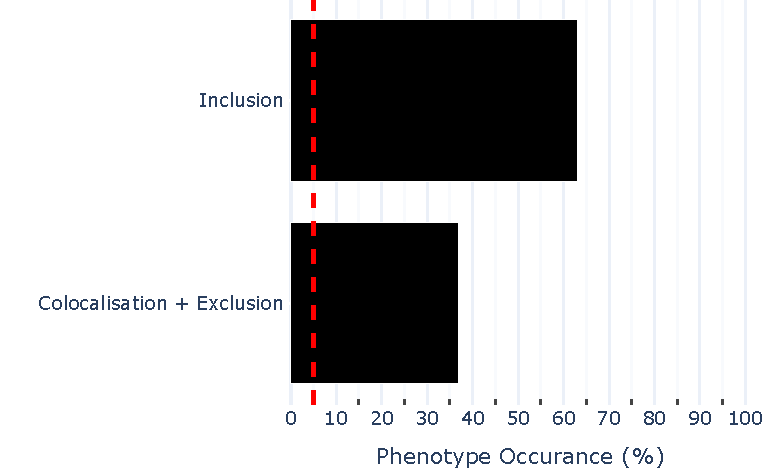
\includegraphics[width=1\linewidth]{09. Chapter 4/Figs/03. pIB/03. IFIT5/01. bar_i5_vero.pdf} 
    \end{subfigure}
    \begin{subfigure}{0.495\textwidth}
        \caption{}
        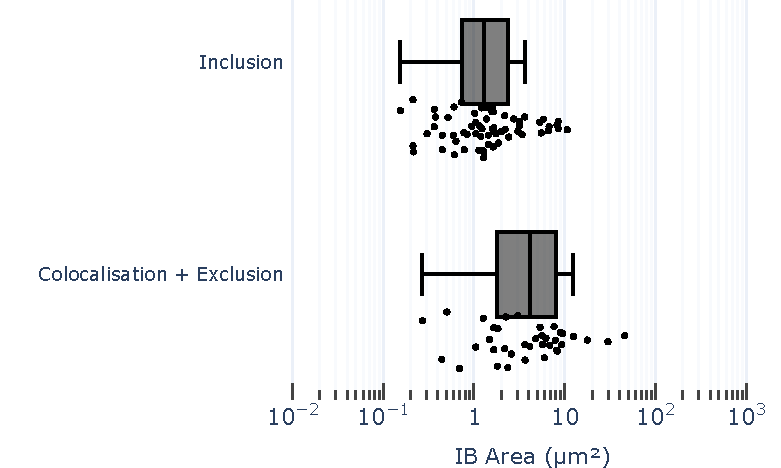
\includegraphics[width=1\linewidth]{09. Chapter 4/Figs/03. pIB/03. IFIT5/02. box_i5_vero.pdf}
    \end{subfigure}
    \begin{subfigure}{1\textwidth}
        \centering
        \caption{}
        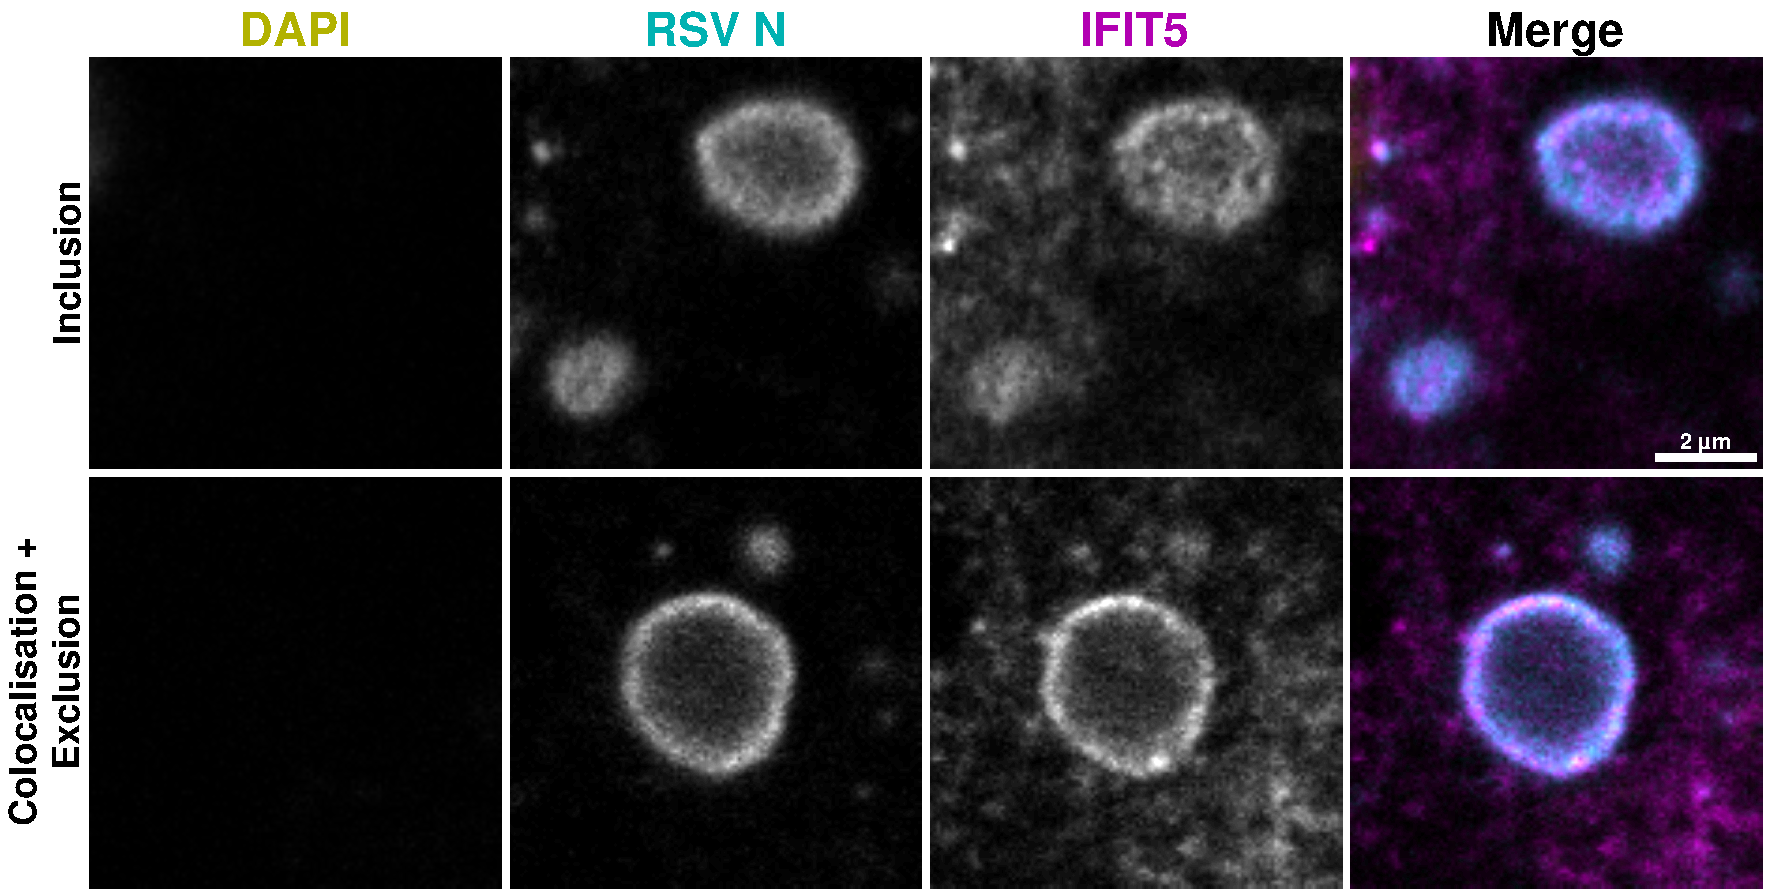
\includegraphics[width=1\linewidth]{09. Chapter 4/Figs/03. pIB/03. IFIT5/03. i5-vero-hnhp.pdf}
    \end{subfigure}
    \caption[i5 vero hnhp]{\textbf{i5 vero hnhp.} 100}
    \label{fig:i5 vero hnhp}
\end{figure}

\subsubsection{Summary} \label{Summary-pib}
Endogenous human IFIT1 seems to be diffused through the human pIB structure. On the other hand, endogenous monkey IFIT1 forms an inclusion in human pIBs, colocalises with the edge of human and bovine pIBs and is excluded from the filamentous pIB network. This suggests that the colocalization is not caused by mere interaction with N or P but its dependant on the integrity of pIBs.

Endogenous monkey IFIT3 seems to be diffuse through the human pIB structures (with maybe a small hint of colocalization).

Endogenous monkey IFIT5 colocalises with human pIBs and with the NP network (this network is never present in infected cells, so we do not know how are other IFIT5s colocalising with it).